%% Copyright 1998 Pepe Kubon
%%
%% `two.tex' --- 2nd chapter for thes-full.tex, thes-short-tex from
%%               the `csthesis' bundle
%%
%% You are allowed to distribute this file together with all files
%% mentioned in READ.ME.
%%
%% You are not allowed to modify its contents.
%%

%%%%%%%%%%%%%%%%%%%%%%%%%%%%%%%%%%%%%%%%%%%%%%%%%
%
%     Chapter 4  
%
%%%%%%%%%%%%%%%%%%%%%%%%%%%%%%%%%%%%%%%%%%%%%%%%

\chapter{A Pruning-based Method On Graph}
\label{ch:graph}

In this section, we will introduce the algorithms to compute the skyline subspace queries. One way to solve this problem is to compute the label distance vectors of all the vertices first and enumerate all the subspaces to check whether the query vertex is a subspace skyline in those subspaces. This method could be very time consuming. In order to make the algorithm more efficient, we manage to avoid some unnecessary computations by applying some pruning techniques in our method. 

\section{BFS Label Collecting}
\label{sec:bfs-collect}
We collect the d-hop labels by Breath-First-Search and get the label vector. The idea is that we start with our query vertex and traverse the graph in the Breath First order. If we visit a vertex with a new label that we have not visited before, we update the entry of that label in \emph{label distance vector} to the distance from query vertex. The Breath First Search process will end if all reachable vertices in $d$ hops has been visited. And we will get the $label distance vector$ of the query vertex when the BFS label collecting ends.

\begin{algorithm}[H]
  \caption{Label Collecting}\label{algo:blah}
  \begin{algorithmic}[1]
  \show\LOOP
    \REQUIRE A graph $G=(V,E)$, a list of label sets $F=\left\{L_v | v \in V\right\}$, the label sets of all vertices, a query vertex $q$, the number of hops $d$;
    \ENSURE The label distance vector $LV_q$ of the query vertex $q$;
    \STATE push $\left(q, 0\right)$ to $Q$
    \WHILE {$Q$ is not empty}
        \STATE $\left( v, dis\right)$ = de-queue $Q$
        \IF{$dis=d$}
            \STATE continue
        \ENDIF
        \FORALL {not visited neighbour $u$ of $v$}
            \STATE push $\left(u, dis+1\right)$ to $Q$
            \FORALL {label $l$ in $L_u$}
                \IF {($l$, $\ast$) not in $LV_q$}
                    \STATE add ($l$, $dis+1$) to $LV_q$
                \ENDIF
            \ENDFOR
        \ENDFOR
    \ENDWHILE
  \end{algorithmic}
\end{algorithm}

\section{Dominating Candidates Set}
\label{sec:bfs-collect}

By collecting the label in $d$ hops from the query vertex, we build the label distance vector of our query vertex. To avoid computing the label distance vectors of all other vertices to find the skyline subspaces, we define a concept of dominating candidates set to compute the skyline subspaces.

\begin{definition}[Dominating Candidates Set]
Given a subspace $\mathcal{B}$, the dominating candidates set of that subspace is the set of vertices that dominate the query vertex $q$ or equal to query vertex $q$ in subspace $\mathcal{B}$, denoted by $\mathit{CAND}_\mathcal{B}$.
\end{definition}

Property~\ref{ppt:empty_cand}, shows that we can determine whether a subspace $\mathcal{B}$ is a \emph{skyline subspace} by checking the elements the \emph{dominating candidates set} of the subspace $\mathcal{B}$.

\begin{property}
\label{ppt:empty_cand}
If $\mathit{CAND}_\mathcal{B} = \emptyset$ or every vertex in $\mathit{CAND}_\mathcal{B}$ is equal to the query vertex $q$ in subspace $\mathcal{B}$, then $q$ is a skyline in subspace $\mathcal{B}$.
\end{property}

\begin{proof}
If $\mathit{CAND}_\mathcal{B} = \emptyset$ or every vertex in $\mathit{CAND}_\mathcal{B}$ is equal to the query vertex $q$ in subspace $\mathcal{B}$, then there is no vertex dominates the query vertex $q$ in $\mathit{CAND}_\mathcal{B}$.
$\mathit{CAND}_\mathcal{B}$ contains all the vertices that are not dominated by $q$. If all the vertices in $\mathit{CAND}_\mathcal{B}$ do not dominate $q$ in $\mathcal{B}$ then $q$ must be a skyline in subspace $\mathcal{B}$.
\end{proof}

\subsection{Dominating Candidates Set of $1$-dimensional subspace}

In this section, we will introduce an algorithm to compute the \emph{dominating candidates set} of $1$-dimensional subspace. We will also introduce the concepts of \emph{Strictly Dominating Subspace} and \emph{Equivalence Subspace} which help us prune the unnecessary dominating candidates.

\begin{definition}[Strictly Dominate]
In a label graph, we say that label distance vector $LV_v=\left\{(l_i, dist_i)\right\}$ dominates label vector $LV_u=\left\{(l_i, dist_i^\prime)\right\}$, if and only if for all i, $dist_i < dist_i^\prime$.
\end{definition}

\begin{definition}[Strictly Dominating Subspace]
Strictly dominating subspace $\mathcal{B}$ is the maximal subspace such that given a vertex $u$, $u_\mathcal{B}$ strictly dominates query vertex $q_\mathcal{B}$ on subspace $\mathcal{B}$.
\end{definition}

\begin{definition}[Equivalence Subspace]
Equivalence subspace $\mathcal{B}$ is the maximal subspace such that given a vertex $u$, if $u_\mathcal{B}$ equals to the query vertex $q_\mathcal{B}$ in subspace $\mathcal{B}$.
\end{definition}

\begin{algorithm}[h]
  \caption{Dominating Candidates Set On $1$-Dimensional Subspace}\label{algo:blah}
  \begin{algorithmic}[1]
  \show\LOOP
    \REQUIRE A graph $G=(V,E)$ and the label vector $LV_q$ of the query vertex $q$;
    \ENSURE Dominating Candidates Set $\mathit{CAND}$ in all one dimension subspace in $LV_q$, $\mathit{EQS}$ and $\mathit{SDS}$;
    \FORALL {$\left(l, dist\right)$ in $LV_q$}
        \FORALL {vertex $v$ contains label $l$}
            \STATE push $\left(v, 0\right)$ to $Q$
        \ENDFOR
        \WHILE {$Q \not= \emptyset$}
            \STATE $\left(v, dist_{v,l}\right)$ = de-queue $Q$
            
            \IF{$dist_{v,l} = dist$}
                \STATE add $\left(u, equal\right)$ to $\mathit{CAND}_l$
                \STATE add $l$ to $\mathit{EQS}_u$
                \STATE continue
            \ENDIF
            \STATE add $\left(u, dom\right)$ to $\mathit{CAND}_l$
            \STATE add $l$ to $\mathit{SDS}_u$
            \FORALL {not visited neighbour $u$ of $v$}
                \STATE push $\left(u, dist_{v,l}+1\right)$ to $Q$
            \ENDFOR
        \ENDWHILE
    \ENDFOR
  \end{algorithmic}
\end{algorithm}

\begin{figure}[h]
    \centering
    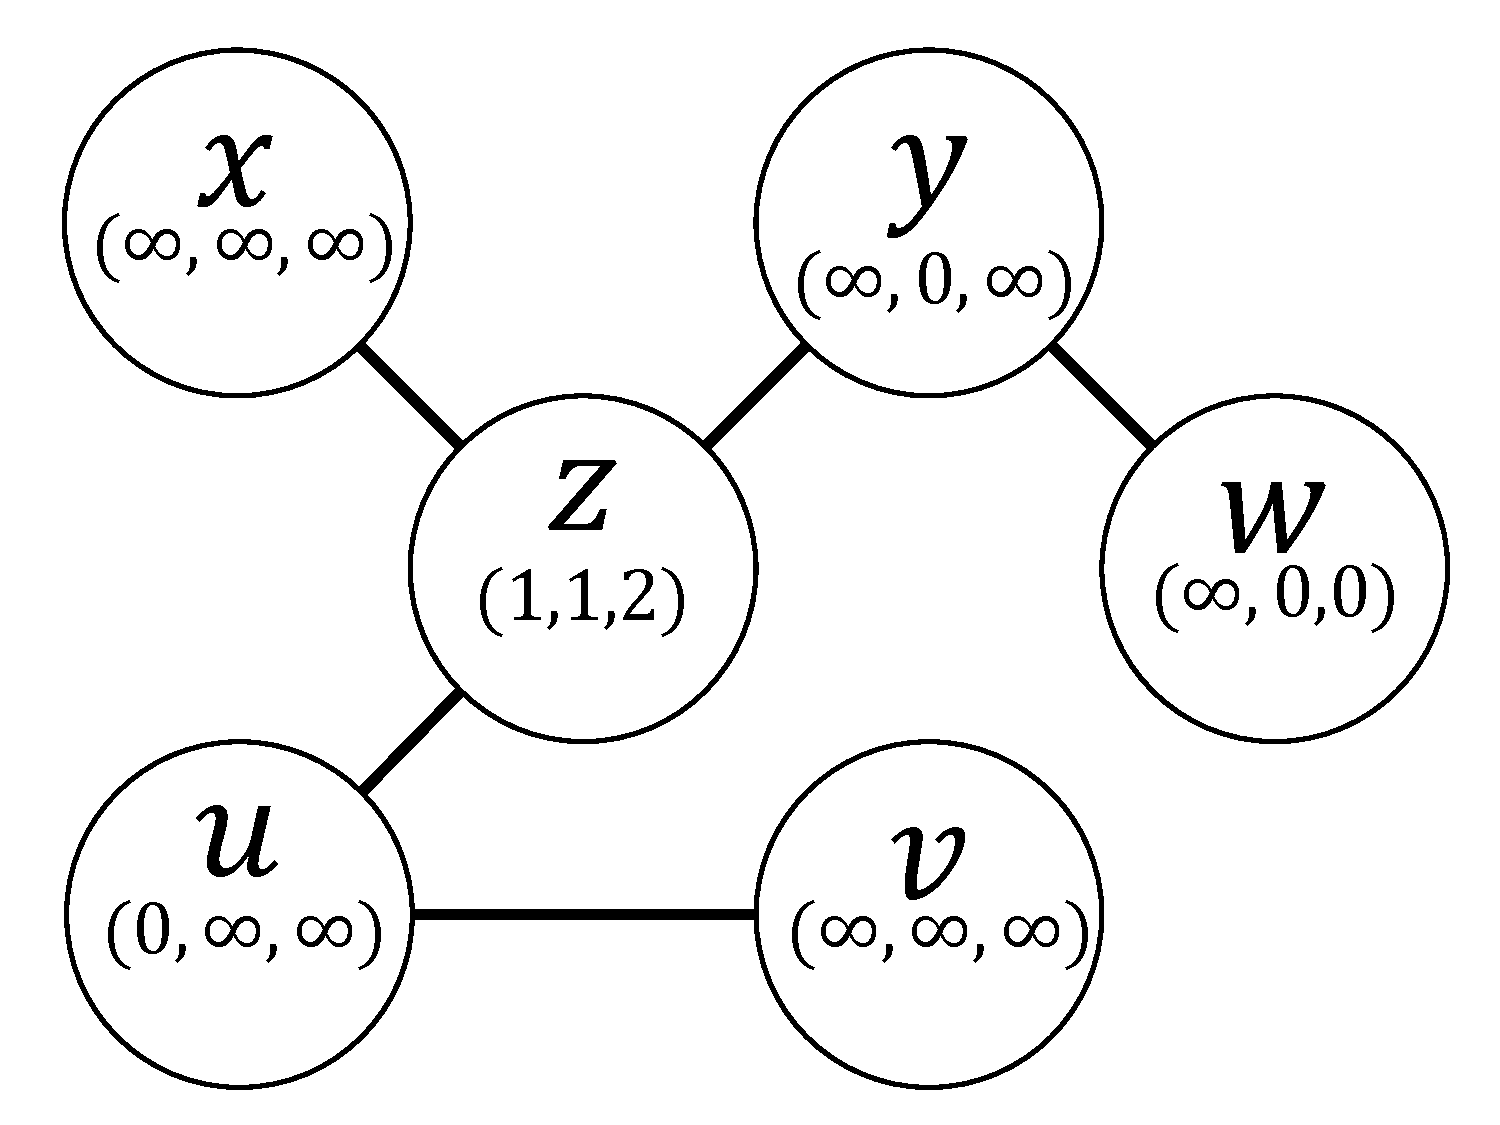
\includegraphics[width=0.5\textwidth]{figs/graph_example_1}
    \caption{\label{font-figure}label distance vector after the first iteration}
    \label{fig:cand_step1}
\end{figure}


\begin{table}[h]
    \centering
    \begin{tabular}{|l|l|l|}
    \hline
      & SDS         & EQS         \\ \hline
    u & A           & $\emptyset$ \\ \hline
    v & $\emptyset$ & $\emptyset$ \\ \hline
    w & BC          & $\emptyset$ \\ \hline
    x & $\emptyset$ & $\emptyset$ \\ \hline
    y & B           & $\emptyset$ \\ \hline
    \end{tabular}
    \caption{\label{font-table}SDS and EQS of each vertex after the first iteration}
\end{table}

\begin{table}[h]
    \centering

    \begin{tabular}{|l|l|}
    \hline
    Subspaces & Dominating Candidates \\ \hline
    A         & $(u, dom)$            \\ \hline
    B         & $(w, dom), (y, dom)$            \\ \hline
    C         & $(w, dom)$            \\ \hline
    \end{tabular}
    \caption{\label{font-table}dominating candidates set of each $1$-dimensional subspace after the first iteration}
\end{table}

\begin{figure}[h]
    \centering
    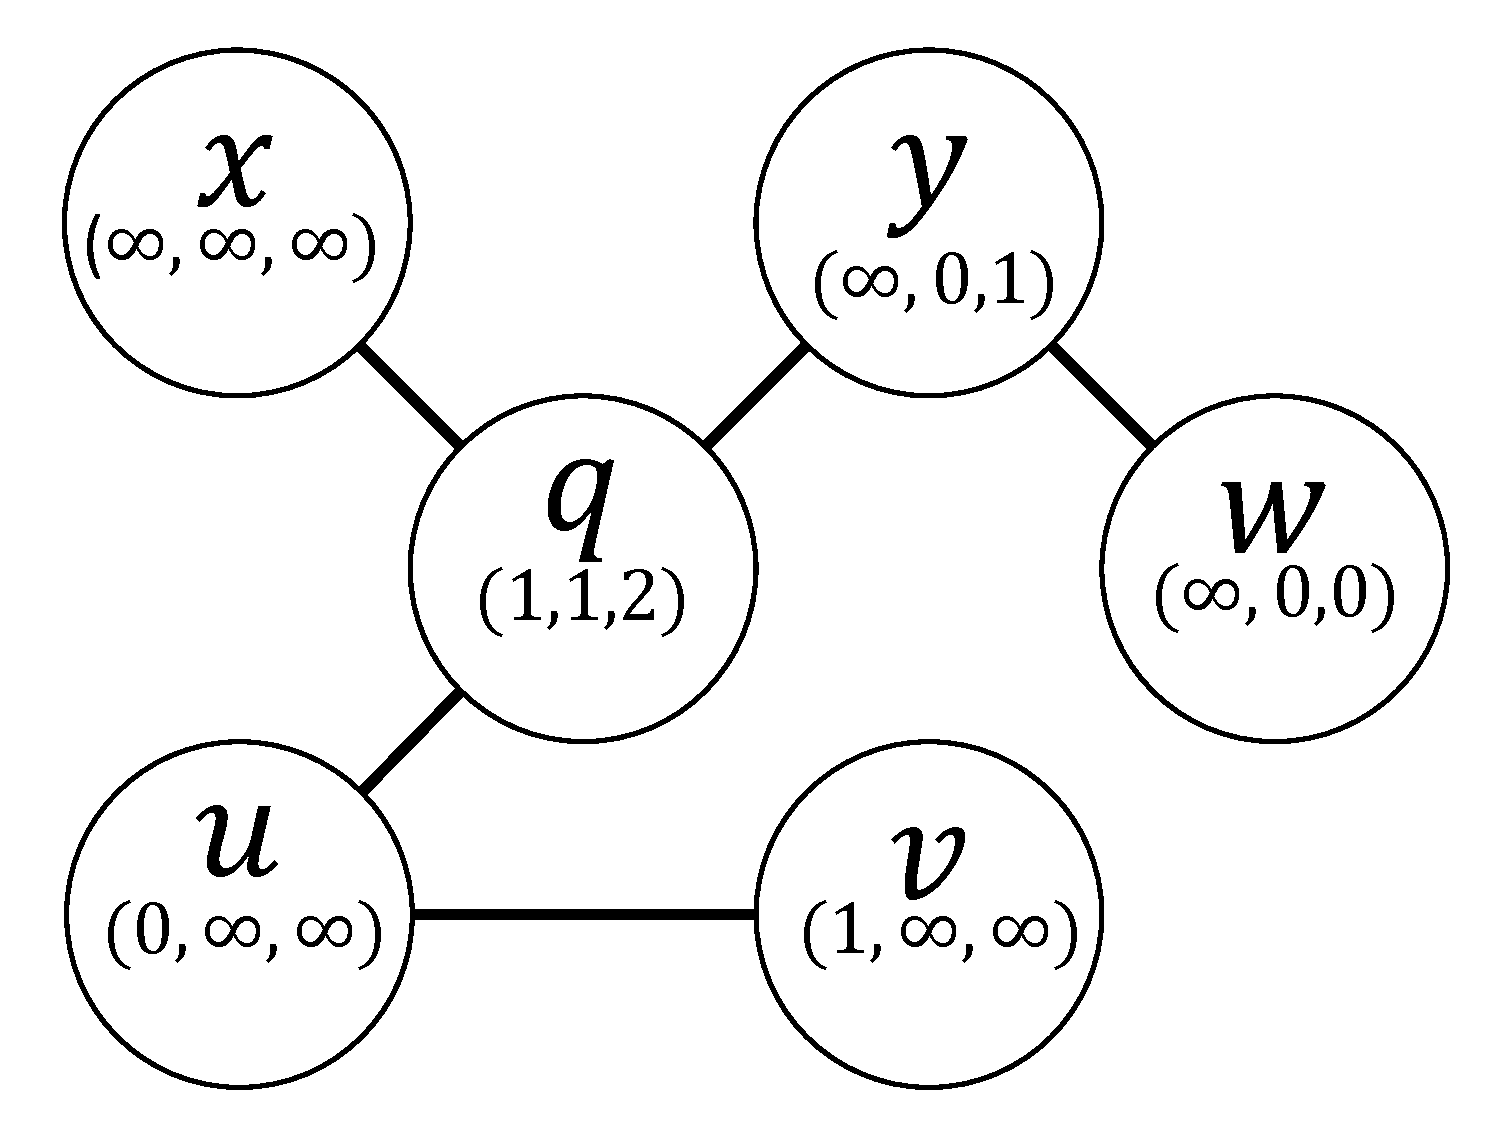
\includegraphics[width=0.5\textwidth]{figs/graph_example_2}
    \caption{\label{font-figure}second iteration of dominating candidates set computation}
    \label{fig:cand_step2}
\end{figure}

\begin{table}[h]
    \centering

    \begin{tabular}{|l|l|l|}
    \hline
      & SDS         & EQS         \\ \hline
    u & A           & $\emptyset$ \\ \hline
    v & $\emptyset$ & A           \\ \hline
    w & BC          & $\emptyset$ \\ \hline
    x & $\emptyset$ & $\emptyset$ \\ \hline
    y & BC          & $\emptyset$ \\ \hline
    \end{tabular}
    \caption{\label{font-table}SDS and EQS of each vertex after the second iteration}
\end{table}

\begin{table}[h]
    \centering

    \begin{tabular}{|l|l|}
    \hline
    Subspaces & Dominating Candidates \\ \hline
    A         & $(u, dom), (v, eq)$            \\ \hline
    B         & $(w, dom), (y, dom)$            \\ \hline
    C         & $(w, dom), (y, dom)$            \\ \hline
    \end{tabular}
    \caption{\label{font-table}dominating candidates set of each $1$-dimensional subspace after the second iteration}
\end{table}






In figure~\ref{tab:distances_graph}, we collect the $3$-hop labels by Breath-First-Search and get the label vector. If a vertex has longer distance from a skill than the distance between that skill and the query vertex then the distance between that vertex and that skill is $\infty$.
\begin{table}[h]
    \centering
    \begin{tabular}{llll}
    \hline
    Distances & A & B & C \\ \hline
    $u$       & 0 & $\infty$ & $\infty$ \\ \hline
    $v$       & 1 & $\infty$ & $\infty$ \\ \hline
    $w$       & $\infty$ & 0 & 0 \\ \hline
    $x$       & $\infty$ & $\infty$ & $\infty$ \\ \hline
    $y$       & $\infty$ & 0 & 1 \\ \hline
    $z$       & 1 & 1 & 2 \\ \hline
    \end{tabular}
    \caption{\label{font-table} distances between each person and each skill in 2-hop}
    \label{tab:d_hops_distance}
\end{table}
We are still able to get the mininmal skyline subspaces of $z$: $(A, B)$ and $(A, C)$ from the Table~\ref{tab:d_hops_distance}.


We define the length of a multiset as the number of elements, including duplicates, in this multiset. Let us denote the lengths of an object and the query as $|X|$ and $|Y|$, respectively. Based on the definition of count-based sliding windows, %we define updates of a query as follows.
%
%
%\begin{definition}[Updates of a query] G
given a query $q=\{e_1, e_2,..., e_{|q|}\}$, the updated query after $u$ time instants is $q'=\{e_{u+1}, e_{u+2}, ..., e_{|q|}, e_{new_1}, e_{new_2}, ..., e_{new_u}\}$, where $u$ is a positive integer and $u<|q|$.
%\end{definition}

To compute the upper bound for Jaccard similarity score after $u$ updates, we can use the following property.
%, whose proof is given in Appendix~\ref{proof:progressive-upper-bound}.

\begin{property}[A Progressive Upper Bound for Jaccard Similarity]%\label{ppt:progressive-upper-bound}
Let $X$, $Y$ be two multisets and $Y_u'$ be the multiset with $u$ updates on $Y$. Given $|X|$, $|Y|$, and the weighted Jaccard similarity score $sim_{Jac}(X, Y)$ between $X$ and $Y$, without the knowledge of the updated elements in $Y_u'$, we have an upper bound for $sim_{Jac}(X, Y_u')$.
% the upper bound for the weighted Jaccard similarity score after $u$ updates 
% $$sim_{Jac}(X, Y_u') \leq \frac{(|X|+|Y|+u)\cdot sim_{Jac}(X, Y)+u}{|X|+|Y|-u\cdot sim_{Jac}(X, Y)-u}.$$

$$sim_{Jac}(X, Y_u') \leq \frac{sim_{Jac}(X, Y)\cdot \alpha+\beta}{\alpha-\beta} = sim_{Jac}(X, Y_u')^{up}$$ where $\alpha = |X| + |Y|$, $\beta = (1+sim_{Jac}(X, Y))\cdot u$
\end{property}

\begin{proof}
By definition, we have $$sim_{Jac}(X, Y) = \frac{\sum_{i=1}^{|\Sigma|} \min\{x_i, y_i\}}{\sum_{i=1}^{|\Sigma|} \max\{x_i, y_i\}}$$ and $\sum_{i=1}^{|\Sigma|} \max\{x_i, y_i\}=|X|+|Y|- \sum_{i=1}^{|\Sigma|} \min\{x_i, y_i\}$. Using the above two equations, we have $$\sum_{i=1}^{|\Sigma|} \min\{x_i, y_i\} =\frac{(|X|+|Y|)\cdot sim_{Jac}(X, Y)}{sim_{Jac}(X, Y)+1}.$$ 

Thus, 
\begin{align*}
& sim_{Jac}(X, Y_u') \\
\leq & \frac{u+\sum_{i=1}^{|\Sigma|} \min\{x_i, y_i\}}{-u+\sum_{i=1}^{|\Sigma|} \max\{x_i, y_i\}} \\
= & \frac{u+\sum_{i=1}^{|\Sigma|} \min\{x_i, y_i\}}{-u+|X|+|Y|-\sum_{i=1}^{|\Sigma|} \min\{x_i, y_i\}} \\
= & \frac{u+\frac{(|X|+|Y|)\cdot sim_{Jac}(X, Y)}{sim_{Jac}(X, Y)+1}}{-u+|X|+|Y|-\frac{(|X|+|Y|)\cdot sim_{Jac}(X, Y)}{sim_{Jac}(X, Y)+1}} \\
= & \frac{(|X|+|Y|+u)\cdot sim_{Jac}(X, Y)+u}{|X|+|Y|-u\cdot sim_{Jac}(X, Y)-u} 
\end{align*}
Let $\alpha = |X| + |Y|$ and $\beta = (1+sim_{Jac}(X, Y))\cdot u$, the upper bound can be simplified as the following.
$$sim_{Jac}(X, Y_u') \leq \frac{sim_{Jac}(X, Y)\cdot \alpha+\beta}{\alpha-\beta} = sim_{Jac}(X, Y_u')^{up}$$ 
\end{proof}

\begin{example}[Computation of Progressive Upper Bound for Jaccard Similarity] 
Let us consider the same multisets $X$ and $Y$ as in Example~\ref{computeSim}. We have $|X|=5$, $|Y|=6$, and $sim_{Jac}(X, Y) = 0.57$. Suppose $u=1$, the upper bound of the Jaccard similarity after an update is $sim_{Jac\_up}(X, Y_1') = 0.85$.
\end{example}

%\subsection{Static Upper Bound Based on Object Lengths} 
%\begin{property}
%(Upper bound for weighted Jaccard similarity).
%Given two multisets $X$ and $Y$ and without loss of generality, suppose their sizes satisfy $|X|\leq|Y|$, the upper bound for the weighted Jaccard similarity score $sim_{Jac}(X, Y)$ is $\frac{|X|}{|Y|}$. 
%\end{property}

%\begin{proof}
%By Definition~\ref{wjacdef}, 
%$$sim_{Jac}(X, Y)=\frac{\sum_{i=1}^{|\Sigma|} \min\{x_i, y_i\}}{\sum_{i=1}^{|\Sigma|} \max\{x_i, y_i\}}$$
%$$\leq \frac{\min\{\sum_{i=1}^{|\Sigma|} x_i, \sum_{i=1}^{|\Sigma|} y_i\}}{\max\{\sum_{i=1}^{|\Sigma|} x_i, \sum_{i=1}^{|\Sigma|} y_i\}}$$ 
%$$=\frac{\min\{|X|, |Y|\}}{\max\{|X|, |Y|\}}=\frac{|X|}{|Y|}.$$
%\end{proof}

\section{A Pruning-based Algorithm (GP)}
\label{sec:pruning-method}

\begin{table}[t]
\centering
\caption{Symbols Used in the Pruning-based Algorithms}
%\small
\begin{tabular}{|l|p{11cm}|} \hline
      Symbol & Interpretation \\ \hline
      $T_i$ & the $i^{th}$ object in a database (DB)\\ \hline
      $m$ & number of objects \\ \hline
      $q_t$ & the query at time $t$ that consists of the elements in the sliding window at time $t$ \\ \hline
      $n$ & size of the sliding window, \emph{i.e.}, query length\\ \hline
      $sim(T_i,T_j)$ & the exact similarity of two objects, $T_i$ and $T_j$\\ \hline
      $sim(T_i, T_j)_{up}$ & the upper bound of similarity score of two objects, $T_i$ and $T_j$\\ \hline
      % $sim(T_i,T_j)_{lo}$ & the lower bound of similarity score of two objects, $T_i$ and $T_j$\\ \hline
      $\Delta sim(T_i)_{+}$ & the maximum increase in similarity score regarding the next query\\ \hline 
      % $\Delta sim(T_i)_{-}$ & the maximum decrease in similarity score regarding the next query\\ \hline 
      % $dis(T_i,T_j)$ & the exact distance of two objects, $T_i$ and $T_j$\\ \hline
      $k$ & number of objects in the result \\ \hline
      $topk_{t}$ & the set of $k$ objects that are most similar to the query at time $t$\\ \hline
      $k^{th}best$ & the $k^{th}$ best result in the current result set\\ \hline
      $v_i$ & the estimated least number of updates needed for object $T_i$ to enter $topk$ \\ \hline
      $u_i$ & a number associated with object $T_i$ indicating in how many steps the current bound for $T_i$ would expire \\ \hline
\end{tabular}
  \label{Symbols}
\end{table}

A brute-force method is to compute the similarity score between the updated query and each object at each time instant, and then sort the scores and get the top-$k$ list. This approach is costly and involves heavy unnecessary computation, since when the query window slides only a small number of positions, e.g., 1 or 2, the changes of the similarity scores are limited. We present a heuristic algorithm that finds the exact top-$k$ objects continuously, as shown in Algorithm~\ref{GPmain}. Table~\ref{Symbols} lists the symbols used in the GP algorithm.

For clearer presentation of our method, let us assume that the arrival of new elements is synchronized with time, \emph{i.e.}, a new element arrives at the stream whenever there is an update in time. The query at time $t+1$ shares a large portion of elements (at least $\frac{n-1}{n}$) with the query at time $t$. Thus, we do not expect a dramatic change in the top-$k$ list, which means that the probability is low that the objects with small similarity scores at time $t$ may enter the top-$k$ list at time $t+1$. We can divide the objects into two categories according to their current similarity scores. In the first category, the similarity scores are small enough so that the objects will not enter the top-$k$ list in the next several updates. The other objects that belong to the second category are regarded as candidates and need to be further verified by computing the exact similarity scores.

For the objects in the first category, there is no need to compute the exact scores in the next time instant. We only need to compute their upper bounds at the next update. If the upper bound of an object is already smaller than the exact similarity scores between the new query and $k$ other objects, then we can safely prune the object. To further reduce computation cost, we only compute bounds for a selected portion of the objects in each update. For each object $T_i$, we estimate $v_i$, the least number of updates needed for an object to enter the top-$k$ list.  We then pick a random integer $u_i$ between $\frac{v_i}{2}$ and $v_i$. We store $u_i$ and the upper bound after $u_i$ updates.  The computation details are described in a subroutine shown in Algorithm~\ref{GPsub}.

 \begin{algorithm2e}[t]
\SetAlgoLined%\small
 \SetKwInput{Input}{Input}
 \SetKwInput{Output}{Output}
 \caption{A General Pruning Algorithm (GP)}
 \label{GPmain}
 \Input{$q_t$; $m$ objects; $topk_{t-1}$; similarity score regarding $q_{t-1}$ or its upper bound for each object; $u_i$ for each object.}
 \Output{$topk_{t}$}
\ForEach{$T_i$ $\in$ $topk_{t-1}$}{
	Compute $sim(T_i, q_t)$ and add to $topk_t$\; 
}
% Compute exact similarity scores for objects in $topk_{t-1}$ regarding $q_t$ and initialize $topk_t$ with the scores\;
 \ForEach{$T_i$ $\not\in$ $topk_{t-1}$}{
  \eIf{$u_i \leq 1$ or $sim(T_i, q_t)_{up} > k^{th}best$}{
   Compute $sim(T_i, q_t)$\; 
   $u_i \gets$ Null\;
   \If{$sim(T_i, q_t) > k^{th}best$}{
   Update $topk_t$\;}
   }
   { 
   $T_i$ is pruned\;
   $u_i \gets u_i - 1$\;
   }
  }
   \ForEach{$T_i$ with $u_i =$ Null}{
   %\If{$u_i =$ Null} 
   $est\_bound\left(sim(T_i, q_t), k^{th}best \right)$\;
 }
\end{algorithm2e} 

In each subsequent update, an object $T_i$ can be pruned if its associated $u_i$ is larger than one and its associated upper bound is no smaller than the $k^{th}$ best score in the current top-$k$ result. We simply decrease $u_i$ by one since the upper bound associated with $T_i$ would expire in $u_i - 1$ updates after the current update. For other objects that are regarded as candidates, we compute the exact similarity score. If the score is greater than the minimum score in the top-$k$ list, this object enters the list and the object with the smallest score in the list leaves. After all the objects are processed once, for each object $T_i$ whose exact similarity is computed at the current time instant, we reset $u_i$ and compute the corresponding upper bound. In fact, in each update, we need to scan through every object, either for decreasing $u_i$, or computing exact similarity. In our algorithm, if an object is said to be pruned in an update, we mean that there is no need to compute the exact similarity for this object regarding the new query.   

\begin{algorithm2e}[t]
 \SetAlgoLined%\small
 \SetKwInput{Input}{Input}
 \SetKwInput{Output}{Output}
  \SetKwInput{Prototype}{Function}
 \caption{Update $u_i$ and Similarity Bounds after Re-computation of Similarity Scores}
\label{GPsub}
\Prototype{$est\_bound(sim(T_i, q_t), k^{th}best)$}
 \Input{$sim(T_i, q_t)$; $k^{th}best$ in $topk_t$; }
 \Output{$u_i; sim(T_i, q_t)_{up}$.}
 
  \eIf{$sim(T_i, q_t) < k^{th}best$}{
  Compute $\Delta sim(T_i)_{+}$\;
  $v_i \gets \lceil \frac{k^{th}best-sim(T_i, q_t)}{\Delta sim(T_i)_{+}}\rceil$\;
  $u_i \gets randint(\frac{v_i}{2}, v_i)$\;
  $sim(T_i, q_t)_{up} \gets $ upper bound after $u_i$ updates\;  
  }
  {$u_i \gets 0$\; $sim(T_i, q_t)_{up} \gets sim(T_i, q_t)$\;}
  Output $u_i$, $sim(T_i, q_t)_{up}$\;
 \end{algorithm2e}
 
 

%This method is illustrated formally in Algorithm~\ref{GPmain}. 
In our implementation, we maintain a min-heap with $k$ elements that stores the top-$k$ objects for efficient updates. Suppose the elements in each object are sorted in a global order, the worst case time complexity of our algorithm is $\mathcal{O}(m\cdot \displaystyle\max_{1 \leq i \leq m}\{n, |T_i|\})$ where $m$ is the number of objects, $n$ is the query length, and $|T_i|$ is the length of the $i^{th}$ object. This worst case happens when no object can be pruned in an update and we need to compute the exact similarity scores between the updated query and all the objects. 
The performance of our pruning-based method is highly related to the similarity score between the evolving query and the $k^{th}$ best object in the top-$k$ result. In each update, we do not need to compute the exact similarity scores for a large portion of the objects, especially when there are exactly $k$ or slightly more than $k$ objects with very high similarity scores while the other objects are very dissimilar to the query. 

%The last thing to mention is about the exactness of this method. 
Finally, we discuss the exactness of this method. To ensure that our method can find the exact top-$k$ objects in each update, we first compute the exact similarity scores between the updated query and each object in the top-$k$ result of the previous query. The top-$k$ list is updated accordingly. The other objects are then processed one by one. The top-$k$ list always consists of the $k$ objects with the largest similarity scores among the objects that have been processed so far. Since the minimum score in the top-$k$ list does not decrease during this process, if the score of an object is smaller than the minimum score in the top-$k$ list when it is processed, it must be smaller than the minimum score of the exact top-$k$ list. Therefore, the algorithm always returns the exact top-$k$ result. 

\section{Generalization to Other Similarity Measures}
\label{sec:gen-sim}
% add applications of edit distance and cosine similarity, reason for extending the method
String similarity search is a fundamental operation in many applications such as data cleaning, information retrieval, and bioinformatics~\cite{DLFL13}. Edit distance is often used to measure the dissimilarity of strings.

Cosine similarity has been widely used for comparing the similarity among documents. A document can be represented by a vector where each component is the frequency of a particular word in the document. This type of term-frequency vector is used in applications including information retrieval, text document clustering, biological taxonomy, and gene feature mapping~\cite{HkP11}.        

To efficiently apply the framework proposed in Section~\ref{sec:pruning-method} to other similarity measures, we need to derive efficient and effective bounds for future updates based on current similarity/distance and its related functions. In this section, we show that the progressive bounds for edit distance, edit similarity, and cosine similarity can be computed in constant time.    

 
\subsection{Edit Distance and Edit Similarity}

\begin{definition}[Edit Distance and Edit Similarity]\label{def:edit-gen}
Given two strings $X$ and $Y$ of length $m$ and $n$ respectively, the edit distance $dis_{ed}(X, Y)$ is the minimum cost required to convert $X$ to $Y$. Typically, we consider three edit operations, namely, insertion, deletion and substitution. The costs of three edit operations, denoted by $\delta_i$, $\delta_d$ and $\delta_s$, are non-negative and can be different. The edit similarity is defined as $$sim_{ed}(X, Y) = 1 - \frac{dis_{ed}(X, Y)}{\max\{\delta_i, \delta_d, \delta_s\}\cdot \max\{|X|, |Y|\}}.$$
\end{definition}

\begin{example}[Computation of Edit Similarity]\label{example:comp-edit}
Suppose the costs of insertion, deletion and substitution are 2, 1, and 3, respectively. $X = ababb$ and $Y = bbabac$ are two strings that consist of symbols in alphabet $\Sigma=\{a, b, c\}$. The edit distance table is shown in Table~\ref{edit01}. From the table, we have $dis_{ed}(X, Y) = 8$. Thus, the edit similarity score between $X$ and $Y$ is $sim_{ed}(X, Y) = 1- \frac{8}{3\times 6} = 0.44$.
\end{example}

\begin{table}[tb]
\caption{Edit distance tables for Example~\ref{example:comp-edit} and Example~\ref{example:bound-ed}}
\label{ed-comp}
\centering
\subfigure[$\delta_i=2, \delta_d=1, \delta_s=3$]{% a
\begin{tabular}{|c||c|c|c|c|c|c|c|} \hline
      &$\epsilon$&b&b&a&b&a&c\\ \hline \hline
      $\epsilon$&0&2&4&6&8&10&12 \\ \hline
      a&1&3&5&4&6&8&10 \\ \hline
      b&2&1&3&5&4&6&8 \\ \hline
      a&3&2&4&3&5&4&6 \\ \hline
      b&4&3&2&4&3&5&7 \\ \hline
      b&5&4&3&5&4&6&8 \\ \hline
    \end{tabular}
    
    \label{edit01}
}
\quad
\subfigure[$\delta_i=\delta_d=\delta_s=1$]{% b
\begin{tabular}{|c||c|c|c|c|c|c|c|} \hline
      &$\epsilon$&b&b&a&b&a&c\\ \hline \hline
      $\epsilon$&0&1&2&3&4&5&6 \\ \hline
      a&1&1&2&2&3&4&5 \\ \hline
      b&2&1&1&2&2&3&4\\ \hline
      a&3&2&2&1&2&2&3\\ \hline
      b&4&3&2&2&1&2&3\\ \hline
      b&5&4&3&3&2&2&3\\ \hline
    \end{tabular}
    
    \label{edit02}
}

\end{table}


Since edit similarity is a function/transformation of edit distance, we first compute the upper and lower bounds for edit distance. We show in Property~\ref{ppt:tri-ineq-ed} that edit distance satisfies triangle inequality. Thus, we can derive the upper and lower bounds of edit distance using triangle inequality as shown in Property~\ref{ppt:bound-ed}. Property~\ref{ppt:bound-es} shows the bounds for edit similarity. 

\begin{property}[Triangle Inequality of Edit Distance~\cite{ChenN04}]\label{ppt:tri-ineq-ed}
Given any three strings $X$, $Y$, and $Z$, the edit distance between $X$ and $Y$ satisfies the following triangle inequality. 
$$dis_{ed}(X,Y) \leq dis_{ed}(X,Z)+dis_{ed}(Z,Y).$$
\end{property}

\begin{proof}
If we want to transform string $X$ into string $Y$, we can first transform $X$ into another arbitrary string $Z$ and then transform $Z$ into $Y$. This kind of two-step edit operation may not have the cheapest cost. Thus, we have $dis_{ed}(X,Y) \leq dis_{ed}(X,Z)+dis_{ed}(Z,Y).$ That is, edit distance satisfies triangle inequality. As shown in Figure~\ref{triIneqa}, we can think of $XY$ to be the shortest path between $X$ and $Y$. An alternative path that consists of two edges $XZ$ and $ZY$ can not have lower cost and this path achieves the same cost as the shortest path if and only if $Z$ falls on $XY$.
% meaning in this case
\end{proof}


\begin{figure}[tb]
\centering
\subfigure[]{% a
\label{triIneqa}
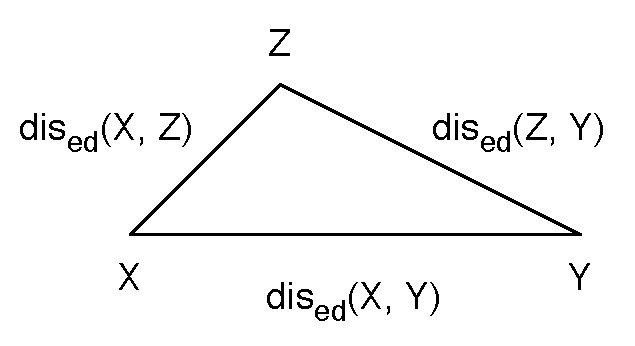
\includegraphics[width=0.4 \textwidth]{fig/triangle01.pdf}}
\quad
\subfigure[]{% b
\label{triIneqb}
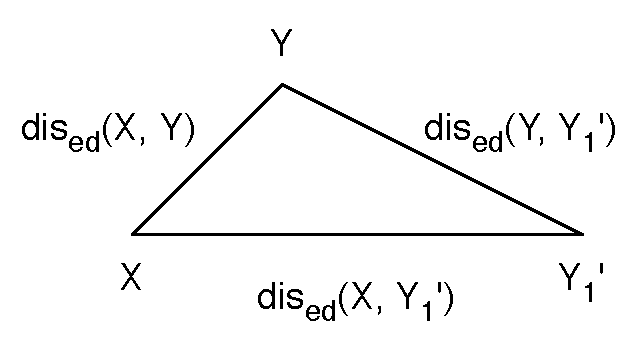
\includegraphics[width=0.4 \textwidth]{fig/triangle02.pdf}}

\caption{Graph Representations for Applying Triangle Inequality}
\label{triIneq}
\end{figure}


\begin{property}[Progressive Bounds for Edit Distance with Unit Penalty Functions]\label{ppt:bound-ed}

Let us consider edit distance with unit penalty functions where the cost for each deletion, insertion, and substitution operation is $1$. Let $X$, $Y$ be two strings and $Y_u'$ be the string with $u$ updates on $Y$. Given the edit distance $dis_{ed}(X, Y)$ between $X$ and $Y$, without the knowledge of the updated elements in $Y_u'$, we have 
$$\max\{0, dis_{ed}(X, Y) - 2u\} \leq dis_{ed}(X, Y_u') \leq dis_{ed}(X, Y) + 2u.$$

\end{property}

\begin{proof}
By the definition of edit distance with unit penalty functions and how queries are updated, we have $dis_{ed}(Y, Y'_1)\in \{0,1,2\}$. Let us consider the following triangle inequalities on a triangle with vertices $X$, $Y$, and $Y_1'$, as shown in Figure~\ref{triIneqb}. 
\begin{align}
dis_{ed}(X, Y'_1) &\leq dis_{ed}(X, Y) + dis_{ed}(Y, Y'_1) \label{ineq01}\\
dis_{ed}(X, Y'_1) &\geq |dis_{ed}(X, Y)-dis_{ed}(Y, Y'_1)| \label{ineq02}
\end{align}

From Inequality~\ref{ineq01},~\ref{ineq02}, and the range of $dis_{ed}(Y, Y'_1)$, we have 
% $$\max\{0, dis_{ed}(X, Y) - 2\} \leq dis_{ed}(X, Y'_1) \leq dis_{ed}(X, Y) + 2.$$ 
\begin{align}\label{ineq03}
\max\{0, dis_{ed}(X, Y) - 2\} \leq dis_{ed}(X, Y'_1) \leq dis_{ed}(X, Y) + 2.
\end{align}

More generally, for edit distance after $u$ updates, we can apply Inequality~\ref{ineq03} $u$ times iteratively and get the bounds as stated in the property.
\end{proof}

\begin{property}[Progressive Bounds for Edit Distance with General Penalty Functions]\label{ppt:bound-ed-gen}

Let us consider edit distance with general penalty functions as discussed in Definition~\ref{def:edit-gen}, where the penalties for insertion, deletion and substitution are denoted as $\delta_i$, $\delta_d$, and $\delta_s$, respectively.  Let $X$, $Y$ be two strings and $Y_u'$ be the string with $u$ updates on $Y$.  Given the edit distance $dis_{ed}(X, Y)$ between $X$ and $Y$, without the knowledge of the updated elements in $Y_u'$, we have 
$$\max\{0, dis_{ed}(X, Y) - u \cdot \max\{\delta_i + \delta_d, \delta_s\} \} \leq dis_{ed}(X, Y_u') \leq dis_{ed}(X, Y) + u \cdot \max\{\delta_i+\delta_d, \delta_s\}\text{.}$$
\end{property}

\begin{proof}
By the definition of edit distance with general penalty functions and how queries are updated, we have $$0 \leq dis_{ed}(Y, Y'_1)\leq \max\{ \delta_i + \delta_d, \delta_s\}\text{.}$$ Let us also apply triangle inequalities on a triangle with vertices $X$, $Y$, and $Y_1'$, as shown in Figure~\ref{triIneqb}. Recalling Inequality~\ref{ineq01} and ~\ref{ineq02} and considering the range of $dis_{ed}(Y, Y'_1)$, we have the following bounds.     
\begin{align}\label{ineq04}
\max\{0, dis_{ed}(X, Y) - \max\{\delta_i + \delta_d, \delta_s\} \} \leq dis_{ed}(X, Y_1') \leq dis_{ed}(X, Y) + \max\{\delta_i+\delta_d, \delta_s\}\text{.}
\end{align}

More generally, for edit distance after $u$ updates, we can apply Inequality~\ref{ineq04} $u$ times iteratively and get the bounds as stated in the property.
\end{proof}


\begin{property}[Progressive Bounds for Edit Similarity with Unit Penalty Functions]\label{ppt:bound-es}

Let us consider edit distance with unit penalty functions where the cost for each deletion, insertion, and substitution operation is $1$. Let $X$, $Y$ be two strings and $Y_u'$ be the string with $u$ updates on $Y$. Given the edit similarity $sim_{ed}(X, Y)$ between $X$ and $Y$, without the knowledge of the updated elements in $Y_u'$, we have 
$$sim_{ed}(X, Y)-\frac{2u}{\max\{|X|, |Y|\}} \leq sim_{ed}(X, Y'_u) \leq \min\{1, sim_{ed}(X,Y)+\frac{2u}{\max\{|X|, |Y|\}}\}.$$
\end{property}

\begin{proof}
By the definition of edit similarity and Property~\ref{ppt:bound-ed}, we have 
\begin{align*} 
sim_{ed}(X, Y'_u) &\leq 1 - \frac{\max\{0, dis_{ed}(X, Y) - 2u\}}{\max\{|X|, |Y|\}}\\
&=\min\{1, sim_{ed}(X,Y)+\frac{2u}{\max\{|X|, |Y|\}}\}\\
sim_{ed}(X, Y'_u) &\geq 1 - \frac{dis_{ed}(X, Y) + 2u}{\max\{|X|, |Y|\}}\\
&= sim_{ed}(X, Y)-\frac{2u}{\max\{|X|, |Y|\}}
\end{align*}
\end{proof}

\begin{property}[Progressive Bounds for Edit Similarity with General Penalty Functions]\label{ppt:bound-es-gen}

Let us consider edit distance with general penalty functions as discussed in Definition~\ref{def:edit-gen}, where the penalties for insertion, deletion and substitution are denoted as $\delta_i$, $\delta_d$, and $\delta_s$, respectively.  Let $X$, $Y$ be two strings and $Y_u'$ be the string with $u$ updates on $Y$.  Given the edit similarity $sim_{ed}(X, Y)$ between $X$ and $Y$, without the knowledge of the updated elements in $Y_u'$, we have 
\begin{align}
sim_{ed}(X, Y'_u) &\geq sim_{ed}(X, Y)-\frac{u\cdot \max\{\delta_i + \delta_d, \delta_s\}}{\max\{\delta_i, \delta_d, \delta_s\} \cdot \max\{|X|, |Y|\}}\\
sim_{ed}(X, Y'_u) &\leq \min\{1, sim_{ed}(X,Y)+\frac{u \cdot \max\{\delta_i + \delta_d, \delta_s\}}{\max\{\delta_i, \delta_d, \delta_s\} \cdot \max\{|X|, |Y|\}}\}.
\end{align}
\end{property}

\begin{proof}
By the definition of edit similarity with general penalty function and Property~\ref{ppt:bound-ed-gen}, we have 
\begin{align*} 
sim_{ed}(X, Y'_u) &\leq 1 - \frac{\max\{0, dis_{ed}(X, Y) - u \cdot \max\{\delta_i + \delta_d, \delta_s\} \}}{\max\{\delta_i, \delta_d, \delta_s\} \cdot \max\{|X|, |Y|\}}\\
&=\min\{1, sim_{ed}(X,Y)+\frac{u \cdot \max\{\delta_i + \delta_d, \delta_s\}}{\max\{\delta_i, \delta_d, \delta_s\} \cdot \max\{|X|, |Y|\}}\}\\
sim_{ed}(X, Y'_u) &\geq 1 - \frac{dis_{ed}(X, Y) + u \cdot \max\{\delta_i + \delta_d, \delta_s\}}{\max\{\delta_i, \delta_d, \delta_s\} \cdot \max\{|X|, |Y|\}}\\
&= sim_{ed}(X, Y)-\frac{u\cdot \max\{\delta_i + \delta_d, \delta_s\}}{\max\{\delta_i, \delta_d, \delta_s\} \cdot \max\{|X|, |Y|\}}
\end{align*}
\end{proof}


\begin{example}[Progressive Bounds for Edit Similarity]\label{example:bound-ed}
Let us consider the same strings $X$ and $Y$ as in Example~\ref{example:comp-edit}. If we use unit penalty functions, the edit distance between $X$ and $Y$ is $3$, as shown in Table~\ref{edit02}. The edit similarity is $1-\frac{3}{1*6}=0.50$. Suppose $u=1$, we have $1 \leq dis_{ed}(X, Y_u') \leq 5$ and $0.167 \leq sim_{ed}(X, Y_u') \leq 0.833$. Let us then consider the general penalty functions where $\delta_i = 2, \delta_d = 1$ and $\delta_s = 3$. As shown in Table~\ref{edit01}, the edit distance between $X$ and $Y$ is $8$. Thus, the edit similarity is $1-\frac{8}{3*6} = \frac{5}{9} = 0.56$. Suppose $u=1$, we have $5 \leq dis_{ed}(X, Y_u') \leq 11$ and $0.39 \leq sim_{ed}(X, Y_u') \leq 0.72$.       
\end{example}


\subsection{Cosine Similarity} 
\begin{definition}[Cosine Similarity]\label{def:cosine}
Let us consider the vector representation mentioned in Chapter~\ref{ch:prob-def}. Given two vectors, $\vec{X}$ and $\vec{Y}$, the cosine similarity is defined using a dot product and magnitudes of vectors. 
\begin{align*}   
sim_{cos}(\vec{X}, \vec{Y}) =\frac{\vec{X} \cdot \vec{Y}} {\| \vec{X} \| \| \vec{Y} \|}=\frac{\sum_{i=1}^{|\Sigma|}\vec{X}_{(i)} \times \vec{Y}_{(i)}}{\sqrt{\sum_{i=1}^{|\Sigma|}(\vec{X}_{(i)})^2} \times \sqrt{\sum_{i=1}^{|\Sigma|}(\vec{Y}_{(i)})^2}}
\end{align*}  
where $\vec{X}_{(i)}$ and $\vec{Y}_{(i)}$ are the $i$-th components of vectors $\vec{X}$ and $\vec{Y}$, respectively.  
\end{definition}

\begin{example}[Computation of Cosine Similarity]\label{example:comp-cos}
Given an alphabet $\Sigma=\{e_1, e_2, e_3, e_4, e_5\}$, $X= \{e_3, e_2, e_2, e_1, e_5, e_2, e_1\}$ and $Y = \{e_1, e_2, e_1, e_3, e_5, e_4, e_2, e_3, e_4\}$ are two multisets over $\Sigma$. We can transform $X$ and $Y$ to vectors, that is, $\vec{X} = \{2, 3, 1, 0, 1\}$ and $\vec{Y} = \{2, 2, 2, 2, 1\}$. We have $\vec{X}\cdot \vec{Y} = 13$, $\|\vec{X}\| = \sqrt{15}$ and $\|\vec{Y}\| = \sqrt{17}$. Thus, $sim_{cos}(\vec{X}, \vec{Y}) = \frac{13}{\sqrt{15}*\sqrt{17}} = 0.81$.  
\end{example}

Given the exact cosine similarity, dot product value of two vectors, and statistics on the current query, we can estimate the cosine similarity after a number of updates in constant time. The following property holds for computing the upper and lower bounds for the updated similarity score.

\begin{property} [Progressive Bounds for Cosine Similarity] 
Let us consider two multi-sets $X$ and $Y$ and their corresponding vector representations $\vec{X}$ and $\vec{Y}$. If the exact cosine similarity between $\vec{X}$ and $\vec{Y}$ is $sim_{cos}(\vec{X}, \vec{Y})$, the dot product value is $\vec{X}\cdot \vec{Y}$, and the value of the maximum component of $\vec{X}$ is $h_{\vec{X}}$, then we have the following bounds for cosine similarity after $u$ updates. Note that we use notations $|Y|$, the cardinality of multi-set $Y$, and $\sum_{i=1}^{|\Sigma|}\vec{Y}_{(i)}$ interchangeably.
\begin{align*} 
sim_{cos}(\vec{X}, \vec{Y}_u') &\geq 
\begin{cases}
\frac{1}{\alpha} \cdot (1-\phi)\cdot sim_{cos}(\vec{X}, \vec{Y}) & , \vec{X}\cdot \vec{Y} \neq 0\\
0 & , \vec{X}\cdot \vec{Y} = 0\\
\end{cases}
\end{align*}

\begin{align*}
sim_{cos}(\vec{X}, \vec{Y}_u') &\leq 
\begin{cases}
\frac{1}{\beta} \cdot (1+\phi)\cdot sim_{cos}(\vec{X}, \vec{Y}) & , \vec{X}\cdot \vec{Y} \neq 0\\
\frac{h_{\vec{X}}\cdot u}{\beta \|\vec{X}\|\|\vec{Y}\|} & , \vec{X}\cdot \vec{Y} = 0\\
\end{cases}
\end{align*} 
where $$\alpha=\sqrt{(2u+1)-\frac{u^2+u}{|Y|}}$$ 
$$\beta=\frac{|Y|}{\sqrt{(|Y|-u)^2+u}}$$ 
and 
$$\phi = \frac{h_{\vec{X}}\cdot u}{\vec{X}\cdot \vec{Y}}\hspace{3 mm},\vec{X}\cdot \vec{Y} \neq 0$$ 
\end{property}

\begin{proof}
Let $\vec{Y}_u'$ be the updated vector of $\vec{Y}$ after $u$ updates. Two inequalities used in this proof are as follows.
\begin{align} 
|Y| &\leq \|\vec{Y}\|^2 \leq |Y|^2 \\
\sqrt{\|\vec{Y}\|^2+u-|Y|^2+(|Y|-u)^2} &\leq \|\vec{Y}_u'\| \leq \sqrt{\|\vec{Y}\|^2-u+|Y|^2-(|Y|-u)^2} 
\end{align}

We first prove the lower bound using the above inequalities.

When $\vec{X}\cdot \vec{Y} \neq 0$,
\begin{align*}
sim_{cos}(\vec{X}, \vec{Y_u'}) &= \frac{\vec{X}\cdot \vec{Y_u'}}{\|\vec{X}\|\|\vec{Y_u'}\|} \geq \frac{(\vec{X}\cdot \vec{Y_u'})_{min}}{(\|\vec{X}\|\|\vec{Y_u'}\|)_{max}}\\ 
&= \frac{\vec{X} \cdot \vec{Y}-h_{\vec{X}}\cdot u}{\| \vec{X} \|\cdot \sqrt{\|\vec{Y}\|^2-u+|Y|^2-(|Y|-u)^2}}\\
&= \frac{\vec{X} \cdot \vec{Y}-h_{\vec{X}}\cdot u}{\frac{\vec{X} \cdot \vec{Y}}{sim_{cos}(\vec{X}, \vec{Y})\cdot \|\vec{Y}\|}\cdot\sqrt{\|\vec{Y}\|^2+2u\cdot |Y|-u^2-u}} \\
&= \frac{\|\vec{Y}\|}{\sqrt{\|\vec{Y}\|^2+2u\cdot |Y|-u^2-u}}(1-\frac{h_{\vec{X}}\cdot u}{\vec{X}\cdot \vec{Y}})sim_{cos}(\vec{X}, \vec{Y})\\
&\geq \frac{1}{\sqrt{1+\frac{2u\cdot |Y|-u^2-u}{|Y|}}}(1-\frac{h_{\vec{X}}\cdot u}{\vec{X}\cdot \vec{Y}})sim_{cos}(\vec{X}, \vec{Y})\\
&= \frac{1}{\alpha}(1-\frac{h_{\vec{X}}\cdot u}{\vec{X}\cdot \vec{Y}})sim_{cos}(X, Y)
\end{align*}
where $\alpha=\sqrt{(2u+1)-\frac{u^2+u}{|Y|}}$. \\ \newline
\indent When $\vec{X}\cdot \vec{Y} = 0$,
\begin{align*}
sim_{cos}(\vec{X}, \vec{Y_u'}) &= \frac{\vec{X}\cdot \vec{Y_u'}}{\|\vec{X}\|\|\vec{Y_u'}\|} \geq \frac{(\vec{X}\cdot \vec{Y_u'})_{min}}{(\|\vec{X}\|\|\vec{Y_u'}\|)_{max}} = 0
\end{align*}



The upper bound can be derived similarly.

When $\vec{X}\cdot \vec{Y} \neq 0$,
\begin{align*}
sim_{cos}(\vec{X}, \vec{Y_u'}) &= \frac{\vec{X}\cdot \vec{Y_u'}}{\|\vec{X}\|\|\vec{Y_u'}\|} \leq \frac{(\vec{X}\cdot \vec{Y_u'})_{max}}{(\|\vec{X}\|\|\vec{Y_u'}\|)_{min}} \\
&= \frac{\vec{X} \cdot \vec{Y}+h_{\vec{X}} \cdot u}{\| \vec{X} \| \cdot \sqrt{\|\vec{Y}\|^2+u-|Y|^2+(|Y|-u)^2}}\\
&= \frac{\vec{X} \cdot \vec{Y}+h_{\vec{X}} \cdot u}{\frac{\vec{X} \cdot \vec{Y}}{sim_{cos}(\vec{X}, \vec{Y}) \cdot \|\vec{Y}\|}\cdot \sqrt{\|\vec{Y}\|^2-2u\cdot |Y|+u^2+u}}\\
&= \frac{\|\vec{Y}\|}{\sqrt{\|\vec{Y}\|^2-2u\cdot |Y|+u^2+u}}(1+\frac{h_{\vec{X}}\cdot u}{\vec{X}\cdot \vec{Y}})sim_{cos}(\vec{X}, \vec{Y})\\
&\leq \frac{1}{\sqrt{1+\frac{u^2+u-2u\cdot |Y|}{|Y|^2}}}(1+\frac{h_{\vec{X}}\cdot u}{\vec{X}\cdot \vec{Y}})sim_{cos}(\vec{X}, \vec{Y})\\
&= \frac{1}{\beta}(1+\frac{h_{\vec{X}}\cdot u}{\vec{X}\cdot \vec{Y}})sim_{cos}(\vec{X}, \vec{Y})
\end{align*}
where $\beta=\frac{|Y|}{\sqrt{(|Y|-u)^2+u}}$. \\ \newline
\indent When $\vec{X}\cdot \vec{Y} = 0$,
\begin{align*}
sim_{cos}(\vec{X}, \vec{Y_u'}) &= \frac{\vec{X}\cdot \vec{Y_u'}}{\|\vec{X}\|\|\vec{Y_u'}\|} \leq \frac{(\vec{X}\cdot \vec{Y_u'})_{max}}{(\|\vec{X}\|\|\vec{Y_u'}\|)_{min}} \\
&= \frac{\vec{X} \cdot \vec{Y}+h_{\vec{X}} \cdot u}{\| \vec{X} \| \cdot \sqrt{\|\vec{Y}\|^2+u-|Y|^2+(|Y|-u)^2}}\\
&\leq \frac{h_{\vec{X}} \cdot u}{\| \vec{X} \|\| \vec{Y} \| \sqrt{1+\frac{u^2+u-2u\cdot |Y|}{|Y|^2}}}\\
&= \frac{h_{\vec{X}}\cdot u}{\beta \|\vec{X}\|\|\vec{Y}\|}
\end{align*}

\end{proof}

\begin{example}[Computation of Progressive Bounds for Cosine Similarity] 
Let us consider the same vectors in Example~\ref{example:comp-cos}. We have $\vec{X}\cdot \vec{Y} = 13$, $h_{\vec{X}}=3$, $|Y|=9$ and $sim_{cos}(\vec{X}, \vec{Y}) = 0.81$. Suppose $u=1$, the upper bound of the cosine similarity after an update is $sim_{cos\_up}(\vec{X}, \vec{Y_1'}) = \frac{\sqrt{65}}{9}*(1+\frac{3}{13})*0.81=0.89$ and the corresponding lower bound is $sim_{cos\_lo}(\vec{X}, \vec{Y_1'}) = \frac{3}{5}*(1-\frac{3}{13})*0.81=0.37$.
\end{example}

Our pruning-based method supports the similarity measures defined above and can be further extended to similarity/distance measures, such as hamming distance, overlap similarity and dice similarity, whose progressive bounds can be computed in constant time.


